%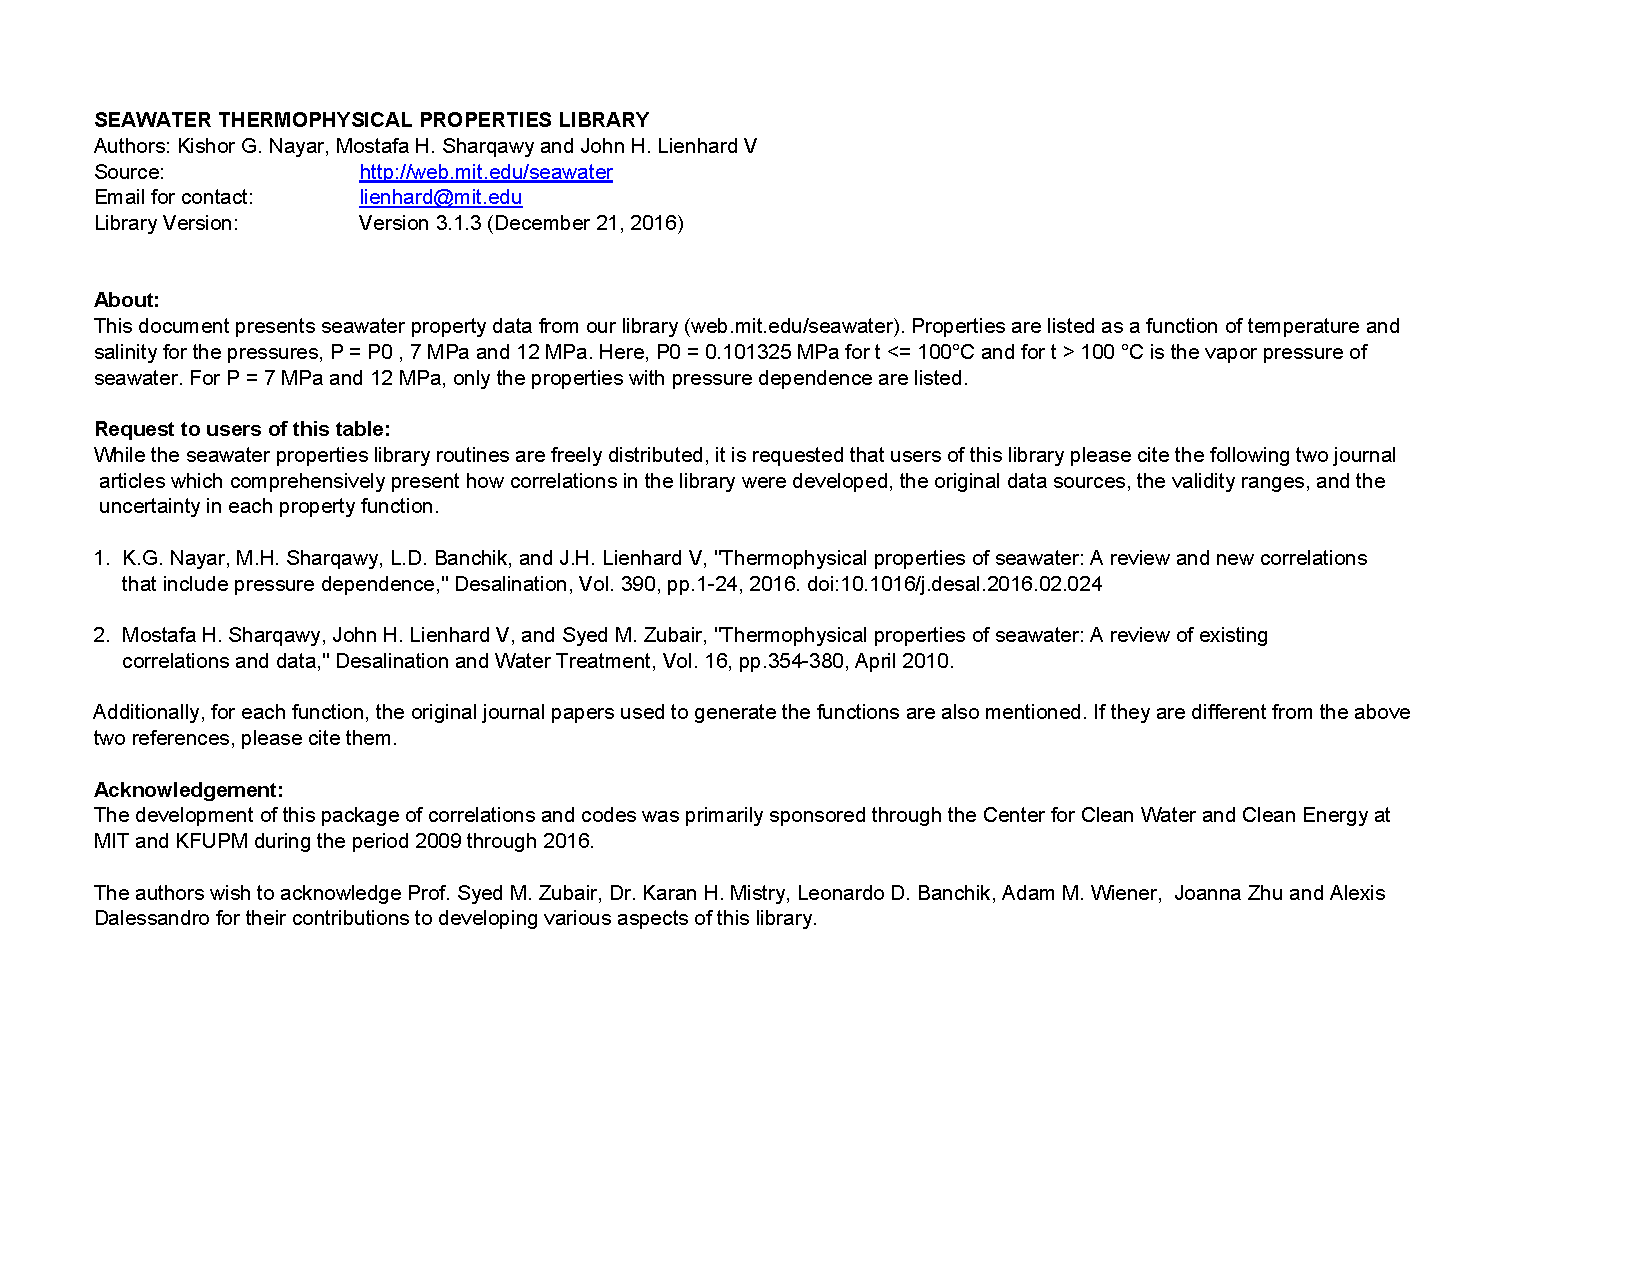
\includepdf[pages=1,pagecommand={\chapter{Propiedades del agua de mar}\label{ch:seawater-properties}\thispagestyle{generalfancy}}]{Content/Appendix/MIT_Seawater_Property_Tables_r2b.pdf}
%
%\includepdf[pages={4,12-13,15,25}, pagecommand={\thispagestyle{generalfancy}}]{Content/Appendix/MIT_Seawater_Property_Tables_r2b.pdf}

\chapter{Propiedades del agua de mar}\label{ch:seawater-properties}

Los datos mostrados en este apéndice son datos distribuidos gratuitamente  gracias a los siguientes artículos de revistas científicas \cites{nayar_thermophysical_2016}{sharqawy_thermophysical_2010}.

	Considerando \(
		P = \begin{cases}
			\qty{101.325}{\kilo\pascal} & \gls{T} \leq \qty{100}{\degreeCelsius} \\
			\text{Presión de vapor de agua} & \gls{T} > \qty{100}{\degreeCelsius} \\
		\end{cases}
	\) para las~\cref{table:Elevación-punto-ebullición,table:Conductividad-térmica-agua-salada,table:Calor-latente-vaporización}

\begin{longtblr}[
	caption = {Elevación del punto de ebullición según su salinidad},
	label = {table:Elevación-punto-ebullición},
	remark{Nota} = {El cambio de temperatura está dado en kelvin}
]{
	colspec = {*{13}{X[c]}},
	cell{1}{1} = {c = 13}{},
	row {1,2} = {
		bg = tabletitleblue,
		fg = white,
		font = \bfseries
	},
	row{even[3]} = {
		bg = tablerowblue
	},
	rowhead = 2,
	width = \linewidth,
	row{3-Z} = {
		font = \footnotesize
	}
}
	Salinidad\\
	{T $\left[\unit{\degreeCelsius}\right]$} 
		& 10 & 20 & 30 & 40 & 50 & 60 & 70 & 80 & 90 & 100 & 110 & 120 \\ 
        0 & 0.067 & 0.138 & 0.213 & 0.291 & 0.373 & 0.458 & 0.547 & 0.64 & 0.736 & 0.836 & 0.939 & 1.046 \\ 
        10 & 0.073 & 0.15 & 0.232 & 0.317 & 0.407 & 0.501 & 0.599 & 0.701 & 0.807 & 0.917 & 1.032 & 1.151 \\ 
        20 & 0.079 & 0.163 & 0.251 & 0.344 & 0.442 & 0.545 & 0.652 & 0.764 & 0.88 & 1.002 & 1.128 & 1.258 \\ 
        30 & 0.085 & 0.176 & 0.272 & 0.373 & 0.479 & 0.59 & 0.707 & 0.829 & 0.956 & 1.088 & 1.225 & 1.368 \\ 
        40 & 0.092 & 0.19 & 0.293 & 0.402 & 0.517 & 0.637 & 0.764 & 0.895 & 1.033 & 1.176 & 1.325 & 1.48 \\ 
        50 & 0.099 & 0.204 & 0.315 & 0.433 & 0.556 & 0.686 & 0.822 & 0.964 & 1.112 & 1.267 & 1.428 & 1.595 \\ 
        60 & 0.106 & 0.219 & 0.338 & 0.464 & 0.597 & 0.736 & 0.882 & 1.035 & 1.194 & 1.36 & 1.532 & 1.711 \\ 
        70 & 0.114 & 0.234 & 0.362 & 0.497 & 0.639 & 0.788 & 0.944 & 1.107 & 1.277 & 1.455 & 1.639 & 1.831 \\ 
        80 & 0.121 & 0.25 & 0.387 & 0.53 & 0.682 & 0.841 & 1.007 & 1.181 & 1.363 & 1.552 & 1.748 & 1.952 \\ 
        90 & 0.129 & 0.267 & 0.412 & 0.565 & 0.726 & 0.895 & 1.072 & 1.257 & 1.45 & 1.651 & 1.86 & 2.076 \\ 
        100 & 0.138 & 0.284 & 0.438 & 0.601 & 0.772 & 0.952 & 1.139 & 1.335 & 1.54 & 1.752 & 1.973 & 2.203 \\ 
        110 & 0.146 & 0.302 & 0.465 & 0.638 & 0.819 & 1.009 & 1.208 & 1.415 & 1.631 & 1.856 & 2.089 & 2.331 \\
\end{longtblr}

\begin{longtblr}[
	caption = {Conductividad térmica del agua según su salinidad},
	label = {table:Conductividad-térmica-agua-salada},
	remark{Nota} = {La conductividad está dada en \unit{\watt\per\m\kelvin}}
]{
	colspec = {*{13}{X[c]}},
	cell{1}{1} = {c = 13}{},
	rowhead = 2,
	row {1,2} = {
		bg = tabletitleblue,
		fg = white,
		font = \bfseries
	},
	row{even[3]} = {
		bg = tablerowblue
	},	
	width = \linewidth,
	row{3-Z} = {
		font = \footnotesize
	}
}
	Salinidad\\
	{T $\left[\unit{\degreeCelsius}\right]$} & 0 & 10 & 20 & 30 & 40 & 50 & 60 & 70 & 80 & 90 & 100 & 110 & 120 \\ 
	0 & 0.572 & 0.571 & 0.57 & 0.57 & 0.569 & 0.569 & 0.568 & 0.568 & 0.567 & 0.566 & 0.566 & 0.565 & 0.565 \\ 
	10 & 0.588 & 0.588 & 0.587 & 0.587 & 0.586 & 0.585 & 0.585 & 0.584 & 0.584 & 0.583 & 0.583 & 0.582 & 0.582 \\ 
	20 & 0.604 & 0.603 & 0.602 & 0.602 & 0.601 & 0.601 & 0.6 & 0.6 & 0.599 & 0.599 & 0.598 & 0.598 & 0.597 \\ 
	30 & 0.617 & 0.617 & 0.616 & 0.616 & 0.615 & 0.615 & 0.614 & 0.614 & 0.613 & 0.613 & 0.612 & 0.612 & 0.611 \\ 
	40 & 0.63 & 0.629 & 0.629 & 0.628 & 0.628 & 0.627 & 0.627 & 0.626 & 0.626 & 0.625 & 0.625 & 0.624 & 0.624 \\ 
	50 & 0.641 & 0.64 & 0.64 & 0.639 & 0.639 & 0.638 & 0.638 & 0.637 & 0.637 & 0.636 & 0.636 & 0.635 & 0.635 \\ 
	60 & 0.65 & 0.65 & 0.649 & 0.649 & 0.648 & 0.648 & 0.647 & 0.647 & 0.647 & 0.646 & 0.646 & 0.645 & 0.645 \\ 
	70 & 0.658 & 0.658 & 0.658 & 0.657 & 0.657 & 0.656 & 0.656 & 0.655 & 0.655 & 0.655 & 0.654 & 0.654 & 0.653 \\ 
	80 & 0.665 & 0.665 & 0.665 & 0.664 & 0.664 & 0.663 & 0.663 & 0.663 & 0.662 & 0.662 & 0.661 & 0.661 & 0.661 \\ 
	90 & 0.671 & 0.671 & 0.67 & 0.67 & 0.67 & 0.669 & 0.669 & 0.669 & 0.668 & 0.668 & 0.667 & 0.667 & 0.667 \\ 
	100 & 0.676 & 0.675 & 0.675 & 0.675 & 0.674 & 0.674 & 0.674 & 0.673 & 0.673 & 0.673 & 0.672 & 0.672 & 0.672 \\ 
	110 & 0.679 & 0.679 & 0.679 & 0.678 & 0.678 & 0.678 & 0.677 & 0.677 & 0.677 & 0.676 & 0.676 & 0.676 & 0.675 \\ 
	120 & 0.682 & 0.681 & 0.681 & 0.681 & 0.68 & 0.68 & 0.68 & 0.679 & 0.679 & 0.679 & 0.679 & 0.678 & 0.678 \\ 
\end{longtblr}


\begin{longtblr}[
	caption = {Calor latente de vaporización del agua según su salinidad},
	label = {table:Calor-latente-vaporización},
	remark{Nota} = {El calor latente de vaporización está dado en \unit{\kilo\joule\per\kg}}
]{
	colspec = {*{13}{X[c]}},
	cell{1}{1} = {c = 13}{},
	rowhead = 2,
	row {1,2} = {
		bg = tabletitleblue,
		fg = white,
		font = \bfseries
	},
	row{even[3]} = {
		bg = tablerowblue
	},	
	width = \linewidth,
	row{3-Z} = {
		font = \scriptsize
	}
}
	Salinidad\\
	{T $\left[\unit{\degreeCelsius}\right]$} & 0 & 10 & 20 & 30 & 40 & 50 & 60 & 70 & 80 & 90 & 100 & 110 & 120 \\ 
	0 & 2500.9 & 2475.9 & 2450.9 & 2425.9 & 2400.9 & 2375.9 & 2350.8 & 2325.8 & 2300.8 & 2275.8 & 2250.8 & 2225.8 & 2200.8 \\ 
	10 & 2477.2 & 2452.5 & 2427.7 & 2402.9 & 2378.1 & 2353.4 & 2328.6 & 2303.8 & 2279 & 2254.3 & 2229.5 & 2204.7 & 2180 \\ 
	20 & 2453.6 & 2429 & 2404.5 & 2379.9 & 2355.4 & 2330.9 & 2306.3 & 2281.8 & 2257.3 & 2232.7 & 2208.2 & 2183.7 & 2159.1 \\ 
	30 & 2429.8 & 2405.5 & 2381.2 & 2356.9 & 2332.6 & 2308.3 & 2284 & 2259.7 & 2235.4 & 2211.1 & 2186.8 & 2162.5 & 2138.2 \\ 
	40 & 2406 & 2381.9 & 2357.9 & 2333.8 & 2309.7 & 2285.7 & 2261.6 & 2237.6 & 2213.5 & 2189.4 & 2165.4 & 2141.3 & 2117.3 \\ 
	50 & 2382 & 2358.1 & 2334.3 & 2310.5 & 2286.7 & 2262.9 & 2239 & 2215.2 & 2191.4 & 2167.6 & 2143.8 & 2120 & 2096.1 \\ 
	60 & 2357.7 & 2334.1 & 2310.5 & 2287 & 2263.4 & 2239.8 & 2216.2 & 2192.7 & 2169.1 & 2145.5 & 2121.9 & 2098.3 & 2074.8 \\ 
	70 & 2333.1 & 2309.8 & 2286.4 & 2263.1 & 2239.8 & 2216.4 & 2193.1 & 2169.8 & 2146.4 & 2123.1 & 2099.8 & 2076.5 & 2053.1 \\ 
	80 & 2308.1 & 2285 & 2261.9 & 2238.8 & 2215.8 & 2192.7 & 2169.6 & 2146.5 & 2123.4 & 2100.4 & 2077.3 & 2054.2 & 2031.1 \\ 
	90 & 2282.6 & 2259.7 & 2236.9 & 2214.1 & 2191.3 & 2168.4 & 2145.6 & 2122.8 & 2100 & 2077.1 & 2054.3 & 2031.5 & 2008.7 \\ 
	100 & 2256.5 & 2233.9 & 2211.3 & 2188.8 & 2166.2 & 2143.7 & 2121.1 & 2098.5 & 2076 & 2053.4 & 2030.8 & 2008.3 & 1985.7 \\ 
	110 & 2229.7 & 2207.4 & 2185.1 & 2162.8 & 2140.5 & 2118.2 & 2095.9 & 2073.6 & 2051.3 & 2029 & 2006.7 & 1984.4 & 1962.1 \\ 
	120 & 2202.1 & 2180.1 & 2158.1 & 2136.1 & 2114.1 & 2092 & 2070 & 2048 & 2026 & 2003.9 & 1981.9 & 1959.9 & 1937.9 \\ 
\end{longtblr}

\begin{figure}[H]
	\centering
	\begin{subfigure}{0.45\linewidth}
		\centering
		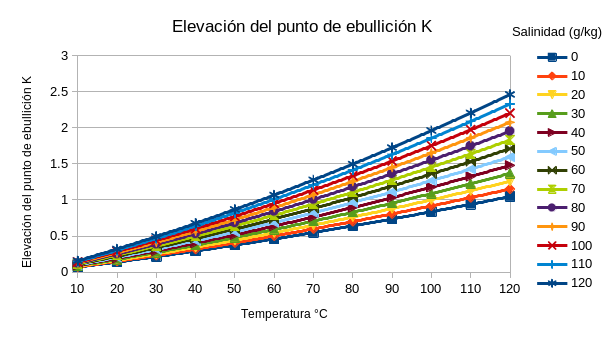
\includegraphics[width=\linewidth, keepaspectratio]{Apéndices/Elevación-punto-ebullición.png}
		\caption{Elevación del punto de ebullición según aumenta la salinidad del agua (\cref{table:Elevación-punto-ebullición})}
		\label{fig:Elevación-punto-ebullición}
	\end{subfigure}
	\hfill
	\begin{subfigure}{0.45\linewidth}
		\centering
		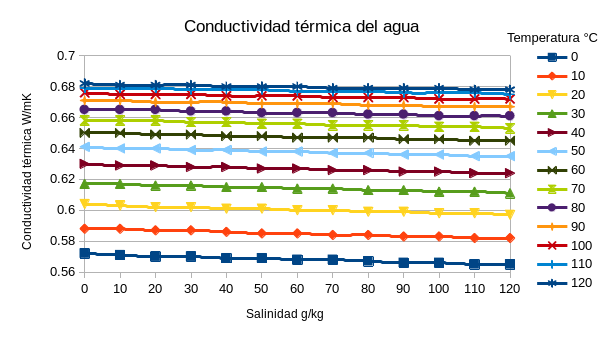
\includegraphics[width=\linewidth, keepaspectratio]{Apéndices/Conductividad-térmica-agua.png}
		\caption{Disminución de la conductividad térmica según aumenta la salinidad del agua (\cref{table:Conductividad-térmica-agua-salada})}
		\label{fig:Conductividad-térmica-agua}
	\end{subfigure}
	\caption{Gráficas del~\cref{ch:seawater-properties}}
	\label{fig:graficas-propiedades-agua-salinidad}
\end{figure}	